\documentclass[11pt]{article}

%encoding
\usepackage[T1]{fontenc}
\usepackage[utf8]{inputenc}
\usepackage{lmodern}

%language
\usepackage[english]{babel}

%paper and text body handling
\usepackage{geometry}
\usepackage{fancyhdr} %Headers and footers
\usepackage{setspace}
\usepackage{lettrine}
\usepackage{glossaries}

%graphics
\usepackage{graphicx}
\graphicspath{{Images/}{./}}
\usepackage[format = plain, labelfont = {bf, it}, textfont = it]{caption}%font settings for captions
\usepackage{xcolor}
\usepackage{pdfpages}
\usepackage{subcaption}
\usepackage{tikz}

%code
%\usepackage{minted}

%math
\usepackage{amsmath}%math
\usepackage{amssymb}%
\usepackage{amsfonts}%
\usepackage{amsthm}%theorems
\usepackage{aligned-overset}
\usepackage{siunitx}
\usepackage{cancel}
\usepackage{braket}
\usepackage{bm}
\usepackage{diffcoeff}
% Use the correct ds in diffs
\difdef{f,s,c}{}{
  op-symbol = \mathrm{d},
}
\difdef{f,s}{f}{
	op-symbol = \delta,
}

%bibliography
\usepackage{csquotes}%for biblatex
\usepackage[
   style = numeric,
   sorting = none,
   date = iso,
   seconds = true
]{biblatex}

%links
\usepackage[colorlinks=true,
            linkcolor=red,
            urlcolor=blue,
            citecolor=gray]{hyperref}

%todo
\usepackage[colorinlistoftodos]{todonotes}

\input{mathCommands}
%text
\makeatletter
   \newlength{\textSize}
   \setlength{\textSize}{\f@size pt}
\makeatother
\setlength{\parindent}{0pt}             % No indentation on new paragraph
\setlength{\parskip}{\textSize}         % Blankline on new paragraph
\setstretch{1.15}


%paper and text body
\geometry{
   a4paper,
   centering,
}


%lettrine settings
\setcounter{DefaultLines}{3}


\newacronym{pml}{PML}{Perfectly Matched Layer}

%bibliography
\addbibresource{sources.bib}

\title{Intresseväckande titel}
\author{David Hambr\ae us}
\date{\textit{\today}}

\begin{document}
\maketitle

\tableofcontents

\printglossaries{}

\section{Introduction}

Something something ``small things are cool''

or something something quantum computers are cool, and they need small
components

Conventionally, when designing these components, the designer comes up with a
design through intuition and parametrizes it with a couple of parameters.
For example she may believe that a structure with periodically placed circular
holes should yield a device that performs the desired function.
% TODO: She? I wrote he first but that will only reinforce the stereotype that
% the are no women in nano science.
The parameters that are unknown might then be the distance between neighbouring
holes and the radius of the holes.
To find the optimal device she would then systematically test parameter values
to see which give the best performance in a simulation of the device.
This brute force method of design limits the possible number of parameters to a
very small number.
If there are 10 different values to test for each parameter, the even 6
parameters would require 1,000,000 simulations.
One can of course use smarter optimization algorithms like bayesian optimization
(cite something, check idas report maybe) or particle swarm optimization (cite the thing the danish guys
cited)
to decrease the number of simulations needed, but it will still be of the same
order.

A different approach that has been gaining some popularity is
\emph{inverse design}. The idea is that if the gradient of the figure of merit
with respect to the parameters can be calculated, then we can use gradient based
optimization methods, which converge much faster, even if the number of
parameters is very large. With these methods, one hopes to be able to search
among a much more general class of designs for the optimal one.
\citeauthor{spins2019} has developed software that successfully uses inverse design for
nanophotonic devices \cite{spins2019}.

With this thesis, we explore the possibility of extending this paradigm to
phononic devices. In order to do so, we attempt to design a phononic beam
splitter.

\subsection{Thesis outline}

\section{Theory}

Maybe some mechanics theory? Linear elastic material etc.
Maybe also mode shape and what the waveguides / mode that we are designing for
is? should that be here? It doesn't really fit in the method section I think...
And more generally how waveguides work?

\subsection{Acoustic waves and waveguides}

\subsection{Adjoint Simulation}

\subsection{Optimization Algorithms}

\section{Methods}

The aim of this thesis is to use inverse design to find a phononic beamsplitter,
a task that can be divided into three parts: First, some definitions of what
should be designed and what constitutes a ``good'' design needs to be made.
Second, we need a way to calculate the gradient of the ``goodness'' with respect
to the design.
And lastly, we need a gradient based optimization algorithm to find the optimal
design.
All of this will be described in this chapter.

\subsection{Design}

The device design to be optimized can be seen in figure~\ref{fig:bs-design}

\begin{figure}[htpb]
	\centering
	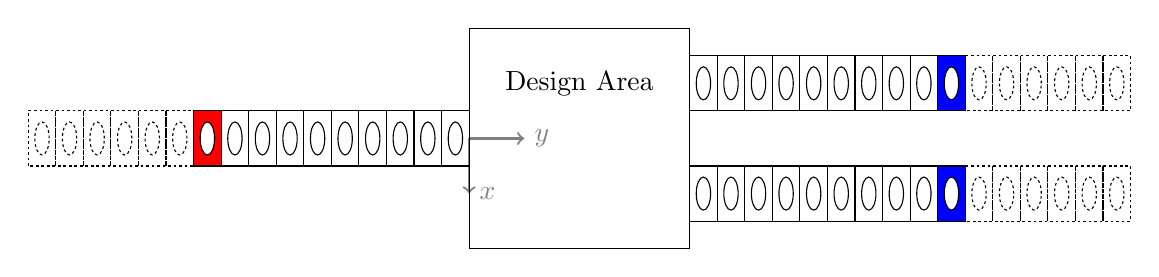
\begin{tikzpicture}[scale=0.7]
	\def \a{0.5}
	\def \w{1.0}
	\def \hx{0.13}
	\def \hy{0.3}
	\def \designx{4.0}
	\def \designy{4.0}
	\def \outputh{1.0}
	\def \nunitcells{16}
	\def \nnonpmls{10}

	% Coordinate system
	\draw[gray, thick, ->] (0,0) -- (0,-1) node [anchor=west] {$x$};
	\draw[gray, thick, ->] (0,0) -- (1,0) node [anchor=west] {$y$};

	% Input waveguide
	\begin{scope}[dash=on 1pt off 1pt phase 0pt]
		\foreach \ix [parse=true] in {-\nunitcells,...,-\nnonpmls-1} {
			\draw (\ix*\a, -0.5*\w) rectangle (\ix*\a + \a, 0.5*\w);
			\draw (\ix*\a + 0.5*\a, 0) circle [x radius=\hx, y radius=\hy];
		}
	\end{scope}
	\foreach \ix in {-\nnonpmls,...,-1} {
		\draw (\ix*\a, -0.5*\w) rectangle (\ix*\a + \a, 0.5*\w);
		\draw (\ix*\a + 0.5*\a, 0) circle [x radius=\hx, y radius=\hy];
	}
	\draw[fill=red] (-\nnonpmls*\a, -0.5*\w) rectangle (-\nnonpmls*\a+\a, 0.5*\w);
	%\node at (-\nnonpmls*\a + 0.5*\a, 0.5*\w) [anchor=south, red] {forward load};
	\draw[fill=white] (-\nnonpmls*\a + 0.5*\a, 0) circle [x radius=\hx, y radius=\hy];

	% Design area
	\draw (0, -\designx / 2) rectangle (\designy, \designx / 2);
	\node at (\designy / 2, 1) {Design Area};

	% Output waveguide
	\foreach \ix [parse=true] in {0, ..., \nnonpmls-1} {
		\draw (\designy + \ix*\a, \outputh - 0.5*\w) rectangle 
			  (\designy + \ix*\a + \a, \outputh + 0.5*\w);
		\draw (\designy + \ix*\a + 0.5*\a, \outputh)
			circle [x radius=\hx, y radius=\hy];

		\draw (\designy + \ix*\a, -\outputh - 0.5*\w) rectangle 
			  (\designy + \ix*\a + \a, -\outputh + 0.5*\w);
		\draw (\designy + \ix*\a + 0.5*\a, -\outputh)
			circle [x radius=\hx, y radius=\hy];
	}
	\begin{scope}[dash=on 1pt off 1pt phase 0pt]
		\foreach \ix [parse=true] in {\nnonpmls, ..., \nunitcells-1} {
			\draw (\designy + \ix*\a, \outputh - 0.5*\w) rectangle 
				  (\designy + \ix*\a + \a, \outputh + 0.5*\w);
			\draw (\designy + \ix*\a + 0.5*\a, \outputh)
				circle [x radius=\hx, y radius=\hy];

			\draw (\designy + \ix*\a, -\outputh - 0.5*\w) rectangle 
				  (\designy + \ix*\a + \a, -\outputh + 0.5*\w);
			\draw (\designy + \ix*\a + 0.5*\a, -\outputh)
				circle [x radius=\hx, y radius=\hy];
		}
	\end{scope}
	\draw[fill=blue] (\designy + \nnonpmls*\a - \a, \outputh-0.5*\w) rectangle
		(\designy + \nnonpmls*\a, \outputh + 0.5*\w);
	\draw[fill=white] (\designy + \nnonpmls*\a - 0.5*\a, \outputh) circle [x radius=\hx, y radius=\hy];
	\draw[fill=blue] (\designy + \nnonpmls*\a - \a, -\outputh-0.5*\w) rectangle
		(\designy + \nnonpmls*\a, -\outputh + 0.5*\w);
	\draw[fill=white] (\designy + \nnonpmls*\a - 0.5*\a, -\outputh) circle [x radius=\hx, y radius=\hy];


\end{tikzpicture}

	\caption{
		Device design to be optimized.
		On the red unit cell, a body load is
		applied that drives a wave traveling right.
		On the blue unit cells is where the output is measured.
		The dashed unit cells are \gls{pml}
	}
	\label{fig:bs-design}
\end{figure}

\subsubsection{Level-set}

Should this section be here?


\subsubsection{Objective function}

\subsection{Adjoint Simulation}

\subsection{Optimization Algorithm}

\section{Conclusions}

\printbibliography{}

\end{document}
